\documentclass[lualatex,ja=standard,a4paper,12pt]{bxjsarticle}
\usepackage{amsmath, amssymb, amsthm}
\usepackage{geometry}
\usepackage{xcolor}
\usepackage{tcolorbox}
\usepackage{booktabs}
\usepackage{array}
\usepackage{graphicx}
\usepackage{listings}

\geometry{margin=25mm}

\tcbuselibrary{theorems, skins, breakable}

\newtcolorbox{defbox}[1]{
  colback=blue!5, colframe=blue!60!black,
  fonttitle=\bfseries, title={#1}, arc=3pt, breakable
}
\newtcolorbox{thmbox}[1]{
  colback=green!5, colframe=green!50!black,
  fonttitle=\bfseries, title={#1}, arc=3pt, breakable
}
\newtcolorbox{pointbox}{
  colback=orange!8, colframe=orange!70!black,
  fonttitle=\bfseries, title={ポイント}, arc=3pt, breakable
}
\newtcolorbox{exbox}[1]{
  colback=gray!6, colframe=gray!50,
  fonttitle=\bfseries, title={例：#1}, arc=3pt, breakable
}
\newtcolorbox{warningbox}{
  colback=red!5, colframe=red!60!black,
  fonttitle=\bfseries, title={注意}, arc=3pt, breakable
}

\lstset{
  basicstyle=\ttfamily\small,
  frame=single,
  framesep=6pt,
  rulecolor=\color{gray!50},
  backgroundcolor=\color{gray!4},
  breaklines=true,
  showstringspaces=false,
  columns=flexible,
}

\title{{\large Hoff 第6章} \\[6pt]
       \textbf{6.2\; Discrete Approximations} \\[4pt]
       {\normalsize （離散近似）ゼミ資料}}
\author{}
\date{}

\begin{document}
\maketitle
\thispagestyle{empty}

% ===========================
\section{この節の位置づけ}
% ===========================

6.1節で，半共役事前分布のもとでは
$\sigma^2$ の\textbf{周辺}事後分布 $p(\sigma^2 \mid y_1, \ldots, y_n)$ が
標準的な分布にならず，直接サンプリングできないことを見た．

\medskip
そこで本節では，まず\textbf{最も素朴な解決策}を試す：
\begin{quote}
「$\theta$ と $\sigma^2$ の値を細かい\textbf{格子（グリッド）}の上に並べて，
各格子点での事後確率を全部計算してしまえばよいのではないか？」
\end{quote}

\noindent これが\textbf{離散近似}（discrete approximation）である．
2パラメータの場合には実際にうまくいく．
しかし最後に見るように，パラメータ数が増えると一瞬で破綻する——
この破綻が，6.3節以降でギブスサンプラーへ向かう本当の動機になる．

\medskip
なお本節以降，Hoff は\textbf{精度}（precision）
\[
  \tilde{\sigma}^2 \;=\; \frac{1}{\sigma^2}
\]
を主役のパラメータとして扱う．事前分布を $1/\sigma^2 \sim \mathrm{Gamma}$ と
おいていたので，精度で書いたほうが式が素直になるためである．

% ===========================
\section{鍵となる事実：正規化定数は知らなくてよい}
% ===========================

ベイズの定理より，同時事後分布は
\[
  p(\theta, \tilde{\sigma}^2 \mid y_1, \ldots, y_n)
  = \frac{p(\theta, \tilde{\sigma}^2,\, y_1, \ldots, y_n)}{p(y_1, \ldots, y_n)}
\]
であり，分母の $p(y_1, \ldots, y_n)$（周辺尤度）は\textbf{パラメータに依存しない}定数である．
したがって，2組のパラメータ値 $\{\theta_1, \tilde{\sigma}_1^2\}$ と
$\{\theta_2, \tilde{\sigma}_2^2\}$ の事後確率の\textbf{比}を取ると分母が約分される：

\begin{align*}
  \frac{p(\theta_1, \tilde{\sigma}_1^2 \mid y_1, \ldots, y_n)}
       {p(\theta_2, \tilde{\sigma}_2^2 \mid y_1, \ldots, y_n)}
  &= \frac{p(\theta_1, \tilde{\sigma}_1^2,\, y_1, \ldots, y_n) \,/\, p(y_1, \ldots, y_n)}
          {p(\theta_2, \tilde{\sigma}_2^2,\, y_1, \ldots, y_n) \,/\, p(y_1, \ldots, y_n)} \\[4pt]
  &= \frac{p(\theta_1, \tilde{\sigma}_1^2,\, y_1, \ldots, y_n)}
          {p(\theta_2, \tilde{\sigma}_2^2,\, y_1, \ldots, y_n)}.
\end{align*}

\begin{pointbox}
事後分布の計算が難しいのは，ほとんどの場合
\textbf{正規化定数 $p(y_1,\ldots,y_n)$ の積分ができない}からであって，
事後分布の「形」が分からないからではない．

\medskip
\textbf{相対確率}だけ分かれば十分な場面（グリッド近似，MCMC）では，
この一番難しい部分を\textbf{丸ごと回避できる}．
6.2節の離散近似も，6.4節以降のギブスサンプラーも，
この同じ一点を利用している．
\end{pointbox}

\medskip
そして同時分布 $p(\theta, \tilde{\sigma}^2, y_1, \ldots, y_n)$ のほうは，
標準的な事前分布と標本分布を掛けただけなので\textbf{簡単に計算できる}：

\begin{align*}
  p(\theta, \tilde{\sigma}^2,\, y_1, \ldots, y_n)
  &= p(\theta, \tilde{\sigma}^2) \times p(y_1, \ldots, y_n \mid \theta, \tilde{\sigma}^2) \\[4pt]
  &= \underbrace{\mathrm{dnorm}(\theta,\, \mu_0,\, \tau_0)}_{\theta \text{ の事前分布}}
   \times \underbrace{\mathrm{dgamma}\!\left(\tilde{\sigma}^2,\, \tfrac{\nu_0}{2},\, \tfrac{\nu_0\sigma_0^2}{2}\right)}_{\tilde{\sigma}^2 \text{ の事前分布}} \\[10pt]
  &\qquad \times \underbrace{\prod_{i=1}^{n} \mathrm{dnorm}\!\left(y_i,\, \theta,\, 1/\sqrt{\tilde{\sigma}^2}\right)}_{\text{尤度}}.
\end{align*}

\noindent ここで事前分布が積に分解できているのは，
6.1節で $\theta$ と $\tilde{\sigma}^2$ を\textbf{事前独立}にしたおかげである
（$p(\theta, \tilde{\sigma}^2) = p(\theta) \times p(\tilde{\sigma}^2)$）．

\begin{pointbox}
\textbf{記法の注意（R 流の書き方）}

Hoff は密度関数を R の関数名でそのまま書く．
\begin{itemize}
  \item $\mathrm{dnorm}(\theta, \mu_0, \tau_0)$：第3引数は\textbf{標準偏差}（分散ではない）
  \item $\mathrm{dnorm}(y_i, \theta, 1/\sqrt{\tilde{\sigma}^2})$：精度 $\tilde{\sigma}^2$ の
        平方根の逆数 $= \sigma$ が標準偏差
  \item $\mathrm{dgamma}(\tilde{\sigma}^2, \nu_0/2, \nu_0\sigma_0^2/2)$：
        第3引数は\textbf{レート}パラメータ（スケールではない）
\end{itemize}
ガンマ分布のパラメータ化は「ガンマ分布・カイ二乗分布補足」の資料を参照．
\end{pointbox}

% ===========================
\section{離散近似の構成}
% ===========================

\begin{defbox}{離散近似（discrete approximation）}
$\{\theta_1, \ldots, \theta_G\}$ と $\{\tilde{\sigma}_1^2, \ldots, \tilde{\sigma}_H^2\}$ を
等間隔に並べたパラメータ値の列とする．
各格子点 $\{\theta_k, \tilde{\sigma}_l^2\}$ に次の事後確率を割り当てる：
\begin{align*}
  p_D(\theta_k, \tilde{\sigma}_l^2 \mid y_1, \ldots, y_n)
  &= \frac{p(\theta_k, \tilde{\sigma}_l^2 \mid y_1, \ldots, y_n)}
          {\sum_{g=1}^{G}\sum_{h=1}^{H} p(\theta_g, \tilde{\sigma}_h^2 \mid y_1, \ldots, y_n)} \\[6pt]
  &= \frac{p(\theta_k, \tilde{\sigma}_l^2,\, y_1, \ldots, y_n) \,/\, p(y_1, \ldots, y_n)}
          {\sum_{g}\sum_{h} p(\theta_g, \tilde{\sigma}_h^2,\, y_1, \ldots, y_n) \,/\, p(y_1, \ldots, y_n)} \\[6pt]
  &= \frac{p(\theta_k, \tilde{\sigma}_l^2,\, y_1, \ldots, y_n)}
          {\sum_{g}\sum_{h} p(\theta_g, \tilde{\sigma}_h^2,\, y_1, \ldots, y_n)}.
\end{align*}
\end{defbox}

\noindent 最後の等式で $p(y_1,\ldots,y_n)$ が約分されているのが要点である．
つまり\textbf{計算できる同時分布をグリッド上で評価して，総和が1になるように割るだけ}でよい．

\medskip
$\theta \in \{\theta_1, \ldots, \theta_G\}$，
$\tilde{\sigma}^2 \in \{\tilde{\sigma}_1^2, \ldots, \tilde{\sigma}_H^2\}$ 上で
総和が 1 になるので，これは\textbf{本物の同時確率分布}である．

\begin{pointbox}
さらに強い解釈がある：
もし $\{\theta, \tilde{\sigma}^2\}$ の同時\textbf{事前}分布が
このグリッド上の離散分布だったとすれば，
$p_D$ は近似ではなく\textbf{厳密な事後分布そのもの}である．

\medskip
つまり「連続事前分布のもとでの事後分布の近似」と見ることも，
「離散事前分布のもとでの正確な事後分布」と見ることもできる．
\end{pointbox}

\paragraph{周辺分布は足し算だけで出る}
同時分布が表の形で手に入れば，周辺分布は\textbf{単に足し合わせる}だけでよい：
\[
  p_D(\theta_k \mid y_1, \ldots, y_n)
  = \sum_{h=1}^{H} p_D(\theta_k, \tilde{\sigma}_h^2 \mid y_1, \ldots, y_n).
\]
6.1節で「積分できない」と嘆いていた周辺化が，
離散化してしまえば\textbf{ただの行・列の合計}になる．
条件付き分布も同様に，1行（1列）を取り出してその和で割るだけで得られる．

\begin{pointbox}
\textbf{なぜヤコビアンを気にしなくてよいか}

連続分布なら $\sigma^2 \to \tilde{\sigma}^2 = 1/\sigma^2$ の変数変換で
ヤコビアン $|d\sigma^2/d\tilde{\sigma}^2| = 1/\tilde{\sigma}^4$ が必要になる．
しかし離散近似では各格子点に\textbf{確率（質量）}を割り当てているので，
点にラベルを付け替えるだけであり，ヤコビアンは出てこない．
$\sigma^2$ 側の分布が欲しければ
格子点のラベルを $1/\tilde{\sigma}_h^2$ に読み替えればよい．
\end{pointbox}

% ===========================
\section{なぜこれが「サンプリングできない」問題の解決になるのか}
% ===========================

ここで一度立ち止まって考えたい．
6.1節の問題は「$p(\sigma^2 \mid y_1,\ldots,y_n)$ が標準的な分布でない」ことだった．
離散近似はその分布に名前を与えたわけではない．
それなのに，なぜ解決になっているのか．

\paragraph{そもそも何のためにサンプリングしたかったのか}
$p(\sigma^2 \mid y_1,\ldots,y_n)$ が標準的な分布でないと困るのは，
\texttt{rgamma()} のような\textbf{乱数生成関数が使えない}からである．
ではなぜ乱数が欲しかったかというと，最終的に知りたいのは
\[
  E[\theta \mid \boldsymbol{y}], \quad
  \mathrm{Var}[\theta \mid \boldsymbol{y}], \quad
  \Pr(\theta > 1.8 \mid \boldsymbol{y}), \quad
  \text{95\% 事後区間}, \quad \ldots
\]
といった\textbf{事後分布についての量}だからである．
これらはすべて事後分布についての\textbf{積分}であり，
モンテカルロ法はその積分を計算するための\textbf{一つの手段}にすぎない．

\begin{pointbox}
\textbf{離散近似は「サンプリングする方法」ではなく「サンプリングせずに済ませる方法」}

パラメータの値を有限個に制限してしまえば，積分はすべて\textbf{有限和}になる．
有限和の計算に「分布の名前」は要らない．足し算は常にできる．
\begin{align*}
  E[\theta \mid \boldsymbol{y}]
  &\;\approx\; \sum_{g=1}^{G} \theta_g \, p_D(\theta_g \mid y_1,\ldots,y_n), \\[4pt]
  \Pr(\theta > 1.8 \mid \boldsymbol{y})
  &\;\approx\; \sum_{g:\,\theta_g > 1.8} p_D(\theta_g \mid y_1,\ldots,y_n).
\end{align*}
\end{pointbox}

\noindent 6.1節で行き詰まった2つの積分が，どちらも足し算に化けていることを確認したい：

\begin{center}
\renewcommand{\arraystretch}{1.8}
\begin{tabular}{lll}
\toprule
 & 連続のまま（6.1節） & 離散化したあと（6.2節） \\
\midrule
正規化定数 & $p(\boldsymbol{y}) = \iint p(\theta,\sigma^2,\boldsymbol{y})\,d\theta\,d\sigma^2$
  & 全セルの和で割るだけ \\
周辺化 & $\int p(\theta, \sigma^2 \mid \boldsymbol{y})\,d\theta$
  & 表の列の足し算 \\
期待値 & $\int \theta\, p(\theta \mid \boldsymbol{y})\,d\theta$
  & 重み付き和 \\
\bottomrule
\end{tabular}
\end{center}

\paragraph{どうしても標本が欲しければ，それも出せる}
さらに言えば，文字通りの「サンプリング」も可能になっている．
確率の表が手に入っているので，
\textbf{セル番号をその確率に従って引けばよい}（R なら \texttt{sample()} 一発）．
カテゴリカル分布からの乱数生成は常に実行できるので，
もとの分布が逆ガンマだったかどうかはもはや関係ない．

\begin{thmbox}{解決の中身}
離散近似は「非標準的な分布からサンプリングする方法を発明した」のではない．
パラメータ空間を有限集合に置き換えることで，
\textbf{分布が標準的である必要そのものをなくした}のである．

\medskip
その代償が，次節で見る2つの問題——
\textbf{グリッドをどこに置くか}と\textbf{次元の呪い}——である．
6.3節以降でサンプリングの路線に戻るのは，この代償が高すぎるからである．
\end{thmbox}

% ===========================
\section{例：ユスリカ（midge）データ}
% ===========================

\begin{exbox}{第5章のユスリカの翅長データ}
データは $n = 9$，$\bar{y} = 1.804$，$s^2 = 0.017$．

\medskip
事前分布の設定：
\begin{itemize}
  \item $\theta$ について：$\mu_0 = 1.9$，$\tau_0 = 0.95$
        （$\theta > 0$ であることは分かっているので，事前質量の大部分が正になるように）
  \item $\sigma^2$ について：$\nu_0 = 1$，$\sigma_0^2 = 0.01$
\end{itemize}

\medskip
\textbf{第5章の共役事前分布との違い}：
共役事前では $\theta$ の事前分散が $\sigma^2/\kappa_0$，
つまり標本分散に比例することを要求された．
標本分散が小さい（このデータでは $s^2 = 0.017$ と非常に小さい）と，
$\theta$ の事前不確実性まで勝手に小さくされてしまうという
望ましくない副作用がある．
半共役事前分布はこの制約から我々を解放し，
$\tau_0 = 0.95$ という「広い」事前不確実性を独立に指定できる．
\end{exbox}

\medskip
グリッドは $100 \times 100$ とし，
\[
  \theta \in \{1.505,\, 1.510,\, \ldots,\, 1.995,\, 2.00\},
  \qquad
  \tilde{\sigma}^2 \in \{1.75,\, 3.5,\, \ldots,\, 173.25,\, 175.0\}
\]
の上で $p(\theta, \tilde{\sigma}^2 \mid y_1, \ldots, y_n)$ を評価する．

\begin{lstlisting}[language=R]
mu0 <- 1.9 ; t20 <- 0.95^2 ; s20 <- .01 ; nu0 <- 1
y <- c(1.64, 1.70, 1.72, 1.74, 1.82, 1.82, 1.82, 1.90, 2.08)

G <- 100 ; H <- 100
mean.grid <- seq(1.505, 2.00, length = G)
prec.grid <- seq(1.75, 175, length = H)
post.grid <- matrix(nrow = G, ncol = H)

for(g in 1:G) {
  for(h in 1:H) {
    post.grid[g,h] <-
      dnorm(mean.grid[g], mu0, sqrt(t20)) *
      dgamma(prec.grid[h], nu0/2, s20*nu0/2) *
      prod(dnorm(y, mean.grid[g], 1/sqrt(prec.grid[h])))
  }
}

post.grid <- post.grid / sum(post.grid)
\end{lstlisting}

\noindent 最後の1行 \texttt{post.grid/sum(post.grid)} が
「正規化定数を積分で求める代わりに，グリッド上の和で代用する」部分である．

\begin{figure}[htbp]
\centering
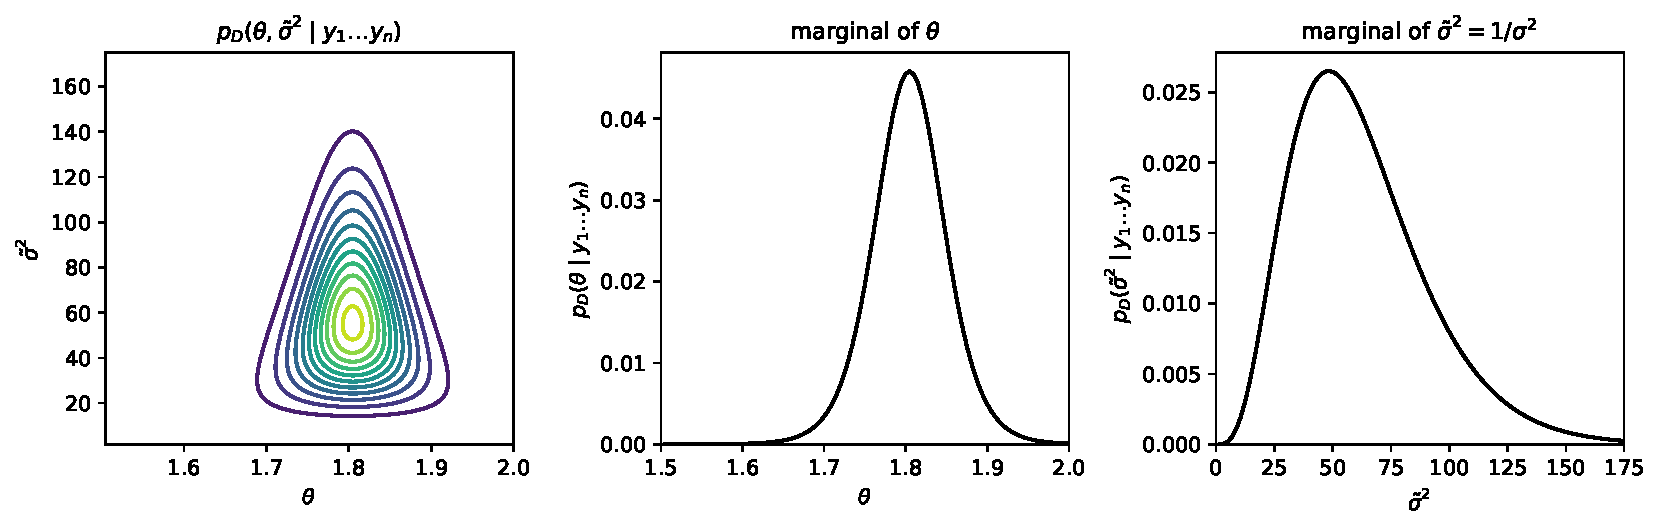
\includegraphics[width=\textwidth]{fig6_1.pdf}
\caption{離散近似による同時事後分布（左）と周辺事後分布（中・右）．
Hoff の Figure 6.1 に対応．}
\end{figure}

\medskip
図の読み取り：
\begin{itemize}
  \item 同時事後分布は $\theta \approx 1.80$，$\tilde{\sigma}^2 \approx 50$
        （すなわち $\sigma^2 \approx 0.02$）あたりに集中している
  \item $\theta$ の周辺事後分布はほぼ対称な山型
  \item $\tilde{\sigma}^2$ の周辺事後分布は右に裾を引いた非対称な形
\end{itemize}

% ===========================
\subsection*{弱点その1：グリッドの範囲を自分で決めなければならない}
% ===========================

上の R コードで \texttt{prec.grid <- seq(1.75, 175, length=H)} と書いたが，
この \textbf{1.75 と 175 という数字はどこから来たのか}．
データからも事前分布からも導かれていない．Hoff が決め打ちしただけである．

\medskip
グリッドとは，計算を始める前に自分で指定する\textbf{有限の箱}である．
箱の置き方を変えると結果がどう変わるかを実際に計算してみる
（$\theta$ 側は固定して $\tilde{\sigma}^2$ の上限だけ動かし，点数は $H=100$ のまま）：

\begin{center}
\renewcommand{\arraystretch}{1.5}
\begin{tabular}{lrrrrr}
\toprule
$\tilde{\sigma}^2$ の範囲 & $E[\tilde{\sigma}^2 \mid \boldsymbol{y}]$
  & 2.5\%点 & 97.5\%点 & 格子幅 & 上端の質量 \\
\midrule
1.75--60（狭すぎ）   & \textbf{40.87} & 15.87 & \textbf{59.41} & 0.59 & \textbf{1.5e-02} \\
1.75--175（Hoff） & 61.78 & 19.25 & 129.50 & 1.75 & 2.5e-04 \\
1.75--3000（広すぎ） & 61.93 & \textbf{32.04} & 122.89 & \textbf{30.29} & 9.6e-88 \\
\bottomrule
\end{tabular}
\end{center}

\paragraph{範囲が狭すぎると（上限 60）}
箱の外にある事後質量は単純に\textbf{捨てられる}．
事後平均が $61.78 \to 40.87$ とずれ，97.5\%点は $59.41$，
つまり\textbf{箱の上端に貼り付いている}．
分布の右の裾がハサミで切られているのだから当然である．

\paragraph{範囲が広すぎると（上限 3000）}
格子点の数 $H$ は 100 のままなので，同じ 100 点を広い範囲に\textbf{ばらまく}ことになる．
格子幅が $1.75 \to 30.29$ と粗くなり，
事後分布の本体（$\tilde{\sigma}^2 \in [30, 100]$ あたり）に入る格子点は
40 点から\textbf{わずか 3 点}に減る．
事後平均は 61.93 とそれらしい値が出るが，
2.5\%点は 32.04（正しくは 19.25）とデタラメであり，
密度のプロットもカクカクになる．

\begin{warningbox}
\textbf{怖いのは，失敗しても出力が正常に見えること}

範囲が狭すぎた場合でも，\texttt{post.grid/sum(post.grid)} が
\textbf{箱の中に残った分を 1 に規格化し直してしまう}．
したがって得られるのは「総和が 1 の，見た目は立派な確率分布」であり，
エラーも警告も一切出ない．
上の 40.87 という誤った事後平均は，何の警告もなく出てくる．

\medskip
\textbf{点検方法：}箱の端（最初と最後の行・列）の確率質量を見ればよい．
上限 175 では $2.5 \times 10^{-4}$ と十分小さいが，
上限 60 では $1.5 \times 10^{-2}$ あり，明らかに切れていると分かる．
\end{warningbox}

\begin{pointbox}
\textbf{循環があることに注意}

よい箱は「質量をほぼ全部含むくらい広く，かつ 100 点で解像できるくらい狭く」
なければならない．
ところが質量がどこにあるかは\textbf{事後分布を見ないと分からず}，
事後分布を見るにはグリッドが要る．

\medskip
2パラメータなら「置く $\to$ 端の質量を見る $\to$ 広げてやり直す」
という試行錯誤で抜け出せる．
しかし10次元では，その試行錯誤を1回まわすこと自体ができない
（次節の次元の呪い）．
\end{pointbox}

% ===========================
\section{弱点その2：次元の呪い}
% ===========================

グリッドの範囲は，2次元なら試行錯誤でなんとかなった．
しかし計算量を見ると，もっと深刻な問題がある．

\medskip
2パラメータで各パラメータを 100 点に区切ると，
格子点の数は $100 \times 100 = 100^2 = 10{,}000$ 個であった．
一般に $p$ 次元の事後分布について同じ細かさの近似を作るには，
$100^p$ 個の事後確率を含む $p$ 次元グリッドが必要になる．

\begin{center}
\renewcommand{\arraystretch}{1.5}
\begin{tabular}{ccl}
\toprule
パラメータ数 $p$ & 格子点数 $100^p$ & 備考 \\
\midrule
1 & $10^{2}$ & 一瞬 \\
2 & $10^{4}$ & 本節の例．一瞬 \\
3 & $10^{6}$ & まだ可能 \\
5 & $10^{10}$ & かなり苦しい \\
10 & $10^{20}$ & 事実上不可能 \\
\bottomrule
\end{tabular}
\end{center}

\begin{warningbox}
\textbf{結論：}
離散近似は\textbf{パラメータ数が少ない密度に対してのみ実行可能}である．

\medskip
しかもベイズ統計で本当に困るのは，
第8章の階層モデルや第9章の回帰のように
パラメータが数十〜数百個ある状況である．
そこでは離散近似は最初から選択肢に入らない．
\end{warningbox}

\begin{pointbox}
\textbf{問題の本質}

グリッド近似は，事後分布の質量がどこにあるかに関係なく
\textbf{パラメータ空間を一様に総なめ}する．
高次元では，事後分布が実際に意味のある確率を持つ領域は
空間全体のごく一部でしかないので，計算のほぼすべてが
「確率ほぼ 0 の点を評価する」ことに費やされる．

\medskip
これに対し次節以降のサンプリング法は，
\textbf{確率の高いところを優先的に訪れる}ように点を打つ．
これが高次元で効く理由である．
\end{pointbox}

% ===========================
\section{まとめと次節への橋渡し}
% ===========================

\begin{thmbox}{6.2節のまとめ}
\begin{enumerate}
  \item 事後分布の\textbf{相対的な}大きさは，同時分布
        $p(\theta, \tilde{\sigma}^2, y_1, \ldots, y_n)$ の比として
        \textbf{計算可能}である（正規化定数 $p(y_1,\ldots,y_n)$ が約分されるため）．

  \item この事実を使い，パラメータ空間のグリッド上で同時分布を評価して
        総和で割れば，事後分布の\textbf{離散近似} $p_D$ が得られる．
        これはグリッド上の正当な確率分布であり，
        離散事前分布を置いたと思えば\textbf{厳密な}事後分布でもある．

  \item 周辺分布・条件付き分布は，表の行や列を\textbf{足す／取り出す}だけで得られる．
        6.1節で問題だった「積分できない周辺化」が有限和に置き換わる．

  \item しかし $p$ 次元には $100^p$ 個の格子点が必要で，
        \textbf{パラメータが少数の場合にしか使えない}．
\end{enumerate}
\end{thmbox}

\paragraph{次節へ}
離散近似の失敗から，方針を変える必要があることが分かった．
6.3節では，もう一度\textbf{完全条件付き分布}に戻る：

\begin{itemize}
  \item $p(\theta \mid \sigma^2, \boldsymbol{y})$ は正規分布（6.1節で確認済み）
  \item $p(\sigma^2 \mid \theta, \boldsymbol{y})$ は——$\theta$ を既知として扱えば——
        逆ガンマ分布になる（6.3節で導出）
\end{itemize}

\noindent どちらも簡単にサンプリングできる．
問題は「両方を同時に扱う方法」だけである．
6.3節ではこの2つを\textbf{交互に使う}アイデアに到達し，
6.4節でそれが\textbf{ギブスサンプラー}として定式化される．

\end{document}
